\documentclass[portrait,a0paper,fontscale=0.29, margin = 8em, final]{baposter}

\usepackage[vlined]{algorithm2e}
\usepackage{times}
\usepackage{calc}
\usepackage{url}
\usepackage{graphicx}
\usepackage{subfig}
\usepackage{float}
\usepackage{amsmath}
\usepackage{amssymb}
\usepackage{relsize}
\usepackage{multirow}
\usepackage{booktabs}
\usepackage{multicol}
\usepackage[T1]{fontenc}
\usepackage{ae}
\usepackage{bm}
\usepackage{microtype}
\usepackage{pst-solides3d}

\graphicspath{{images/}}

 %%%%%%%%%%%%%%%%%%%%%%%%%%%%%%%%%%%%%%%%%%%%%%%%%%%%%%%%%%%%%%%%%%%%%%%%%%%%%%%%
 %%%% Some math symbols used in the text
 %%%%%%%%%%%%%%%%%%%%%%%%%%%%%%%%%%%%%%%%%%%%%%%%%%%%%%%%%%%%%%%%%%%%%%%%%%%%%%%%
 % Format
 \newcommand{\RotUP}[1]{\begin{sideways}#1\end{sideways}}
\newcommand{\ud}{\,\mathrm{d}}
\newcommand{\rulesep}{\unskip\ \vrule\ }
 %%%%%%%%%%%%%%%%%%%%%%%%%%%%%%%%%%%%%%%%%%%%%%%%%%%%%%%%%%%%%%%%%%%%%%%%%%%%%%%%
 % Multicol Settings
 %%%%%%%%%%%%%%%%%%%%%%%%%%%%%%%%%%%%%%%%%%%%%%%%%%%%%%%%%%%%%%%%%%%%%%%%%%%%%%%%
 \setlength{\columnsep}{0.7em}
 \setlength{\columnseprule}{0mm}


 %%%%%%%%%%%%%%%%%%%%%%%%%%%%%%%%%%%%%%%%%%%%%%%%%%%%%%%%%%%%%%%%%%%%%%%%%%%%%%%%
 % Save space in lists. Use this after the opening of the list
 %%%%%%%%%%%%%%%%%%%%%%%%%%%%%%%%%%%%%%%%%%%%%%%%%%%%%%%%%%%%%%%%%%%%%%%%%%%%%%%%
 \newcommand{\compresslist}{
 \setlength{\leftmargin}{0pt}
 \setlength{\itemsep}{0pt}
 \setlength{\parskip}{0pt}
 \setlength{\parsep}{0pt}
 }

%%%%%%%%%%%%%%%%%%%%%%%%%%%%%%%%%%%%%%%%%%%%%%%%%%%%%%%%%%%%%%%%%%%%%%%%%%%%%
%% Begin of Document
%%%%%%%%%%%%%%%%%%%%%%%%%%%%%%%%%%%%%%%%%%%%%%%%%%%%%%%%%%%%%%%%%%%%%%%%%%%%%
\begin{document}
%%%%%%%%%%%%%%%%%%%%%%%%%%%%%%%%%%%%%%%%%%%%%%%%%%%%%%%%%%%%%%%%%%%%%%%%%%%%%
%% Here starts the poster
%%---------------------------------------------------------------------------
%% Format it to your taste with the options
%%%%%%%%%%%%%%%%%%%%%%%%%%%%%%%%%%%%%%%%%%%%%%%%%%%%%%%%%%%%%%%%%%%%%%%%%%%%%
\begin{poster}{
 % Show grid to help with alignment
 grid=false,
 % Column spacing
 colspacing= 1em,
 columns=3,
 % backgroud color
 background=shadetb,
 bgColorTwo=black!5!white!90!,
 bgColorOne=white,
 % Color style
 headerColorOne=red!20!white!95!yellow,
 borderColor=red!50!white!95!yellow,
 % Format of textbox
 boxColorOne=white,
 textborder=rectangle,
 % Format of text header
 headerborder=open,
 headershape=roundedright,
 headershade=plain,
 headerheight=0.12\textheight}
 % university logo
 {
      \raisebox{0em}[5em][0em]{
\includegraphics[scale = 0.7]{GM-logo.png}}
 }
 % Title
 {\sc Spatio-temporal modelling for \\ \vspace{0.2em} global sea level change}
 % Author
 {Zhe Sha,  Maike Schumancher,  William Llovel, \\ 
 Jonathan Rougier and Jonathan Bamber
 \\
  \vspace{0.1em}
 {University of Bristol}\\
 \hspace{-2em} 
\noindent\makebox[\linewidth][c]{
\includegraphics[width = 1.1\paperwidth]{seplines}}
}
 % department logo
 {
  %\begin{tabular}{r}
    \raisebox{0em}[3em][0em]{
\includegraphics[scale = 0.21]{UoB-logo-colour.jpg}}
    %\raisebox{0em}[0em][0em]{\includegraphics[height=0.03\textheight]{oulogo}}
  %\end{tabular}

 }


%%%%%%%%%%%%%%%%%%%%%%%%%%%%%%%%%%%%%%%%%%%%%%%%%%%%%%%%%%%%%%%%%%%%%%%%%%%%%%
%%% Now define the boxes that make up the poster
%%%---------------------------------------------------------------------------
%%% Each box has a name and can be placed absolutely or relatively.
%%% The only inconvenience is that you can only specify a relative position
%%% towards an already declared box. So if you have a box attached to the
%%% bottom, one to the top and a third one which should be inbetween, you
%%% have to specify the top and bottom boxes before you specify the middle
%%% box.
%%%%%%%%%%%%%%%%%%%%%%%%%%%%%%%%%%%%%%%%%%%%%%%%%%%%%%%%%%%%%%%%%%%%%%%%%%%%%%

%%%%%%%%%%%%%%%%%%%%%%%%%%%%%%%%%%%%%%%%%%%%%%%%%%%%%%%%%%%%%%%%%%%%%%%%%%%%%%
  \headerbox{1. Introduction and framework}{name=intro,column=0,row=0, span = 3}{
  \setlength{\columnsep}{10pt}
  \begin{multicols}{3}
  \textbf{Motivation}
  
Future sea level rise (SLR) is one of the most serious consequences of climate change. Traditionally, the Earth system components that contributes to SLR were treated separately and often led to inconsistencies between discipline-specific estimates of each part of the sea level budget.

Our project aims at producing a physically-based, data-driven solution for the complete coupled land-ocean-solid Earth system that is consistent with the full suite of observations, prior knowledge and fundamental geophysical constraints.

\begin{figure}[H]
\centering
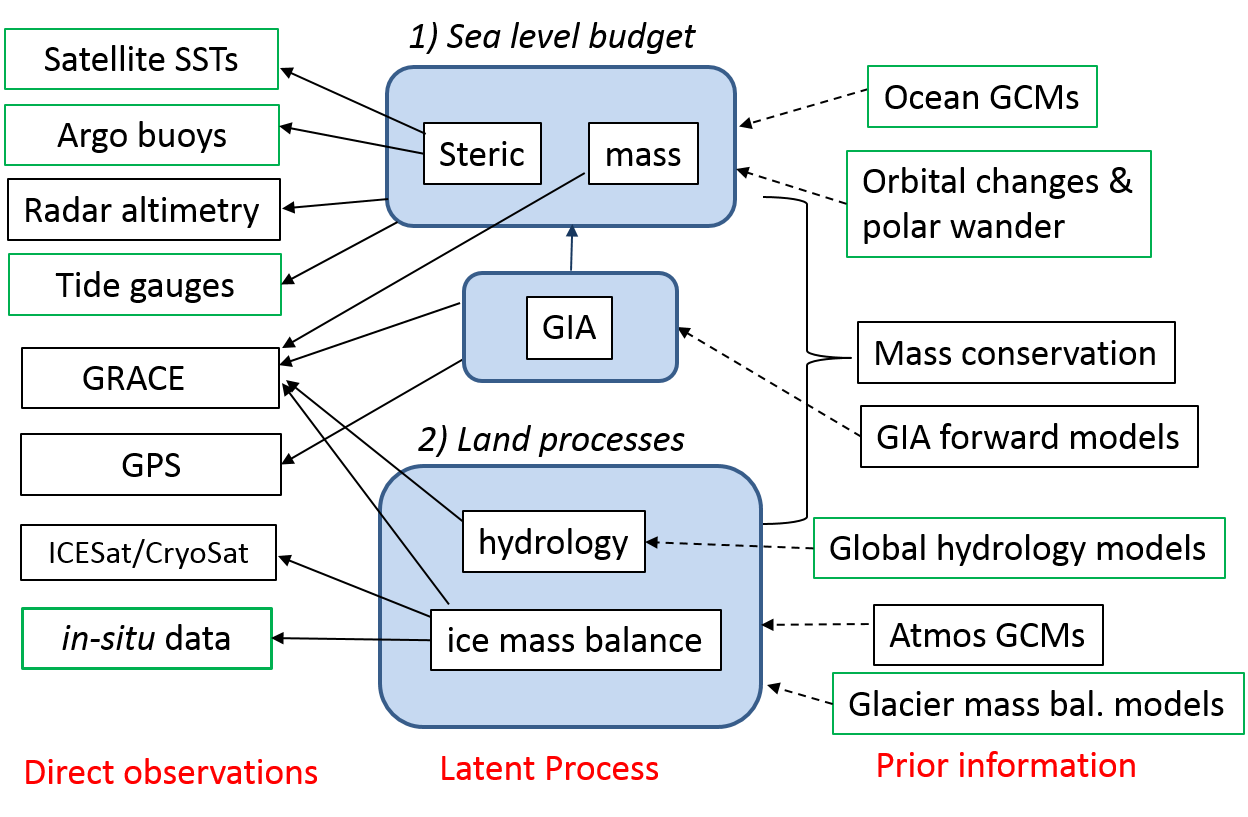
\includegraphics[width = 0.36\textwidth]{BHM}
\caption{BHM framework for solving SLR}
\end{figure}


\begin{center}
\textbf{Bayesian Hierarchical Model (BHM)}
\end{center}
\begin{align*}
\bm{y} | \bm{\beta}, \bm{x}, \bm{\theta} &\sim \mathcal{N}(\bm{P}(\bm{\beta}) \bm{x}, \bm{\Sigma_{obs}}), \\
\bm{x} | \mathcal{A}, \bm{X}, \bm{\theta} &\sim \mathcal{N}(\mathcal{A}\bm{X}, \bm{Q}^{-1}(\bm{\theta})),\\
\bm{X(\bm{s})} | \bm{\theta}, &\sim \mathcal{GP} (\bm{\mu}(\bm{s}), k(\bm{s}, \bm{r}; \bm{\theta})), \\
\bm{\beta} &\sim \mathcal{N}(\bm{\mu}_{\bm{\beta}}, \bm{\Sigma}_{\bm{\beta}}),\\
f(\bm{\theta}) &\sim \mathcal{N}(\bm{\mu}_{\bm{\theta}}, \bm{\Sigma}_{\bm{\theta}}).
\end{align*}
\hspace{2em}where $\mathcal{A}$ is a linear operator that maps physical process $\bm{X}$ into the observation space and $\bm{P}$ represents the relationship between the observations and the latent processes.
\end{multicols}
}
%%%%%%%%%%%%%%%%%%%%%%%%%%%%%%%%%%%%%%%%%%%%%%%%%%%%%%%%%%%%%%%%%%%%%%%%%%%%%%
  \headerbox{2. Big data challenges}{name=data,column=0,span = 3, below = intro }{
  
 \begin{minipage}{0.35\textwidth}
\begin{itemize}
\begin{figure}[H]
\centering
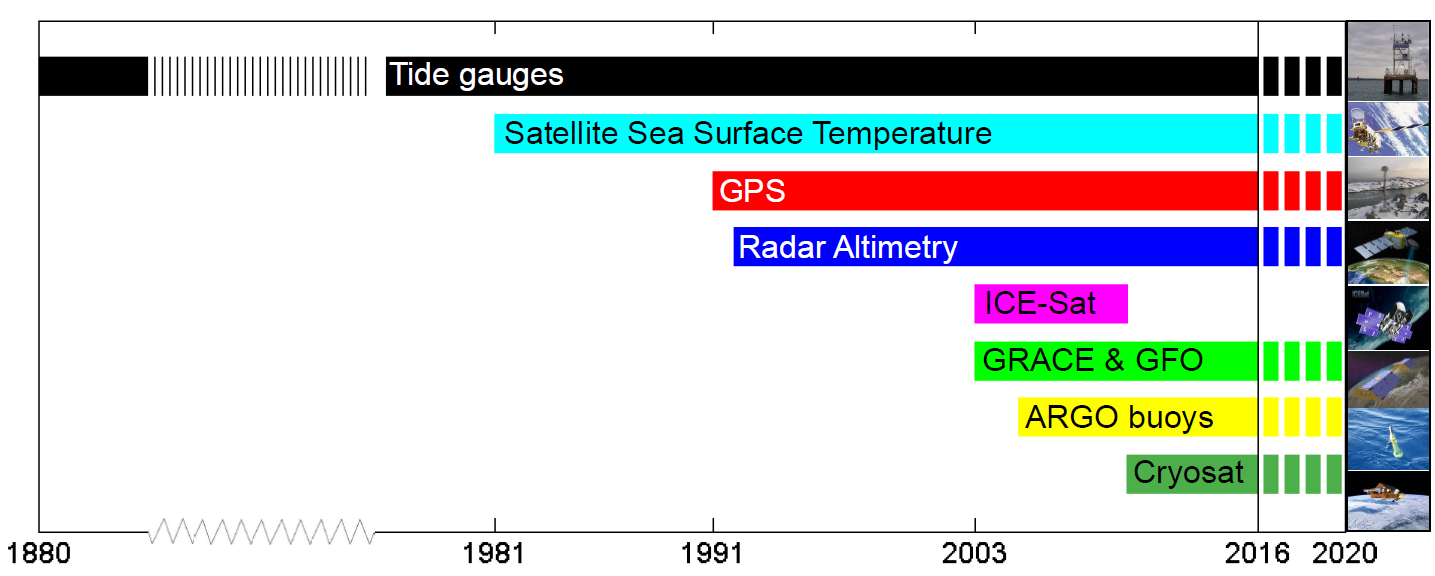
\includegraphics[width =\textwidth]{data}
\caption{Temporal coverage of the observations.}
\end{figure}

 \setlength{\itemsep}{0pt}
\item Massive volume of data sets with uncertainty in error estimates.
\item Inconsistent temporal coverages and frequencies between the data sets.
\item In-situ and satellite measurements exhibit various spatial footprints.
\item Different spatially-varying mesh grids in high resolutions for SPDE approximation.
\end{itemize}
\end{minipage}
\begin{minipage}{0.65\textwidth}
\begin{figure}[H]
\centering
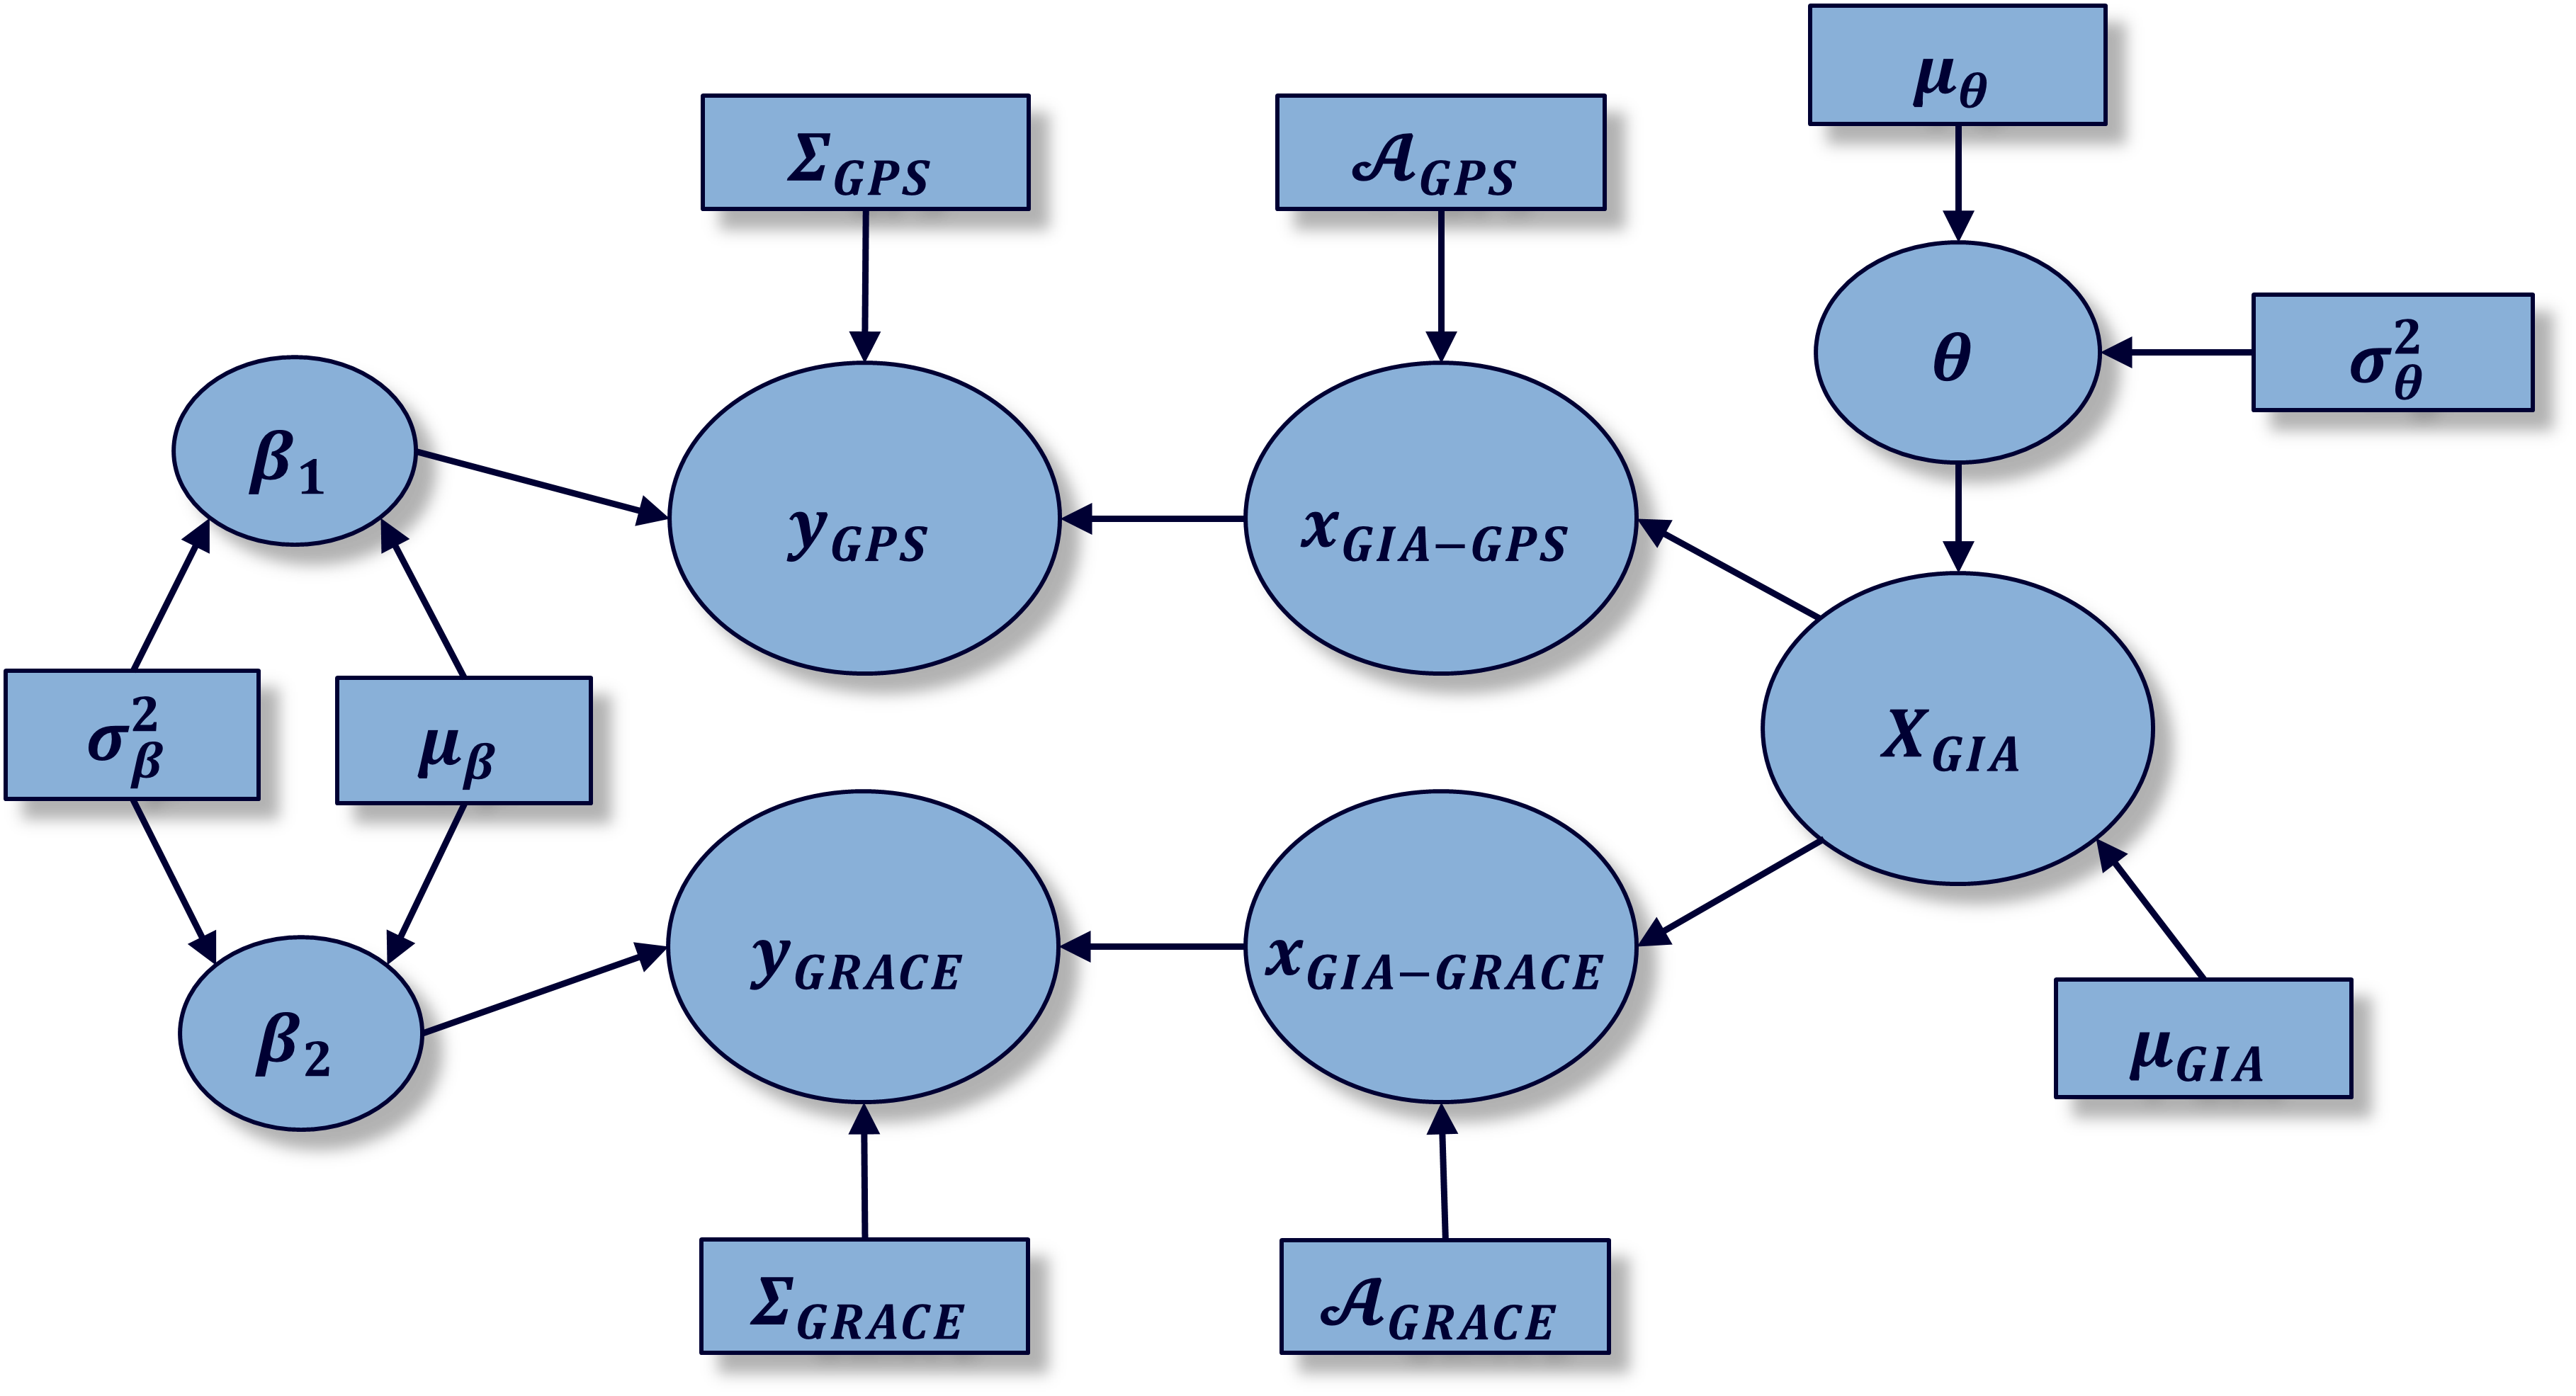
\includegraphics[width = 0.8\textwidth]{graph}
\caption{Graphical model for the GIA.}
\end{figure}
\end{minipage}
  }
  %%%%%%%%%%%%%%%%%%%%%%%%%%%%%%%%%%%%%%%%%%%%%%%%%%%%%%%%%%%%%%%%%%%%%%%%%%%%%%
\headerbox{3. Example: the glacio-isostatic adjustment (GIA)}{name=result,column = 0, span = 2,
 below = data}{
\begin{multicols}{2}
%\includegraphics[trim = 10 0 0 0, scale = 0.5, clip = true]{resid}
%\includegraphics[trim = 10 0 0 0, scale = 0.5, clip = true]{resid2}
\end{multicols}
With my current design of implementation, the approximation to (\ref{eq:1})
is not accurate enough and show a substantial variability. Therefore, only the
fitting of the residual obtained from a GLM model is presented here.

\vspace{0.5em}
The approximate MLEs of are $\rho = 0.2308, \; \sigma^2 = 0.7028$, and they can be reused for
constructing weights in GLM. Note the range of $\rho$ is about
$(-0.25,0.25)$. The estimated $\rho$ shows a strong positive correlation.


 }

  %%%%%%%%%%%%%%%%%%%%%%%%%%%%%%%%%%%%%%%%%%%%%%%%%%%%%%%%%%%%%%%%%%%%%%%%%%%%%%
  \headerbox{4. Future Work}{name=future,column=2, below = data}{
\begin{itemize}\compresslist
\item Assume presence-only data \cite{Bhatt2013}
\item Joint modelling the 277 species
\item Occurrences collected at lower resolution with substantial variation in
  explanatory variables over the region
\item Occurrence data collected at different resolutions  \cite{Bhatt2013}
\item Elaboration of the spatial covariance structure
\end{itemize}

  }
  %%%%%%%%%%%%%%%%%%%%%%%%%%%%%%%%%%%%%%%%%%%%%%%%%%%%%%%%%%%%%%%%%%%%%%%%%%%%%%


\headerbox{References}{name=ref,column=0, span = 2, below=result}{

\renewcommand{\refname}{\vspace{-1em}}
\bibliographystyle{abbrv}
\bibliography{references,ecoapp}

  }
  %%%%%%%%%%%%%%%%%%%%%%%%%%%%%%%%%%%%%%%%%%%%%%%%%%%%%%%%%%%%%%%%%%%%%%%%%%%%%%
\headerbox{Acknowledgement}{name=ack,column=2,below=future}{
Funded by the European Research Council (ERC) under the European Union's Horizon 2020 research and innovation programme under grant agreement No 69418
\begin{figure}[H]
  \centering
  \begin{tabular}{c|c}
    \subfloat{
\includegraphics[width = 0.3\textwidth]{EUflag}} \hspace{1em} &
    \hspace{1em} \subfloat{
\includegraphics[width = 0.3\textwidth]{ERClogo}}
  \end{tabular}
\end{figure}


}
 %%%%%%%%%%%%%%%%%%%%%%%%%%%%%%%%%%%%%%%%%%%%%%%%%%%%%%%%%%%%%%%%%%%%%%%%%%%%%%
\headerbox{Keep in touch}{name=contact,column=2,below=ack}{
Website: www.globalmass.eu 

Email: globalmass-project@bristol.ac.uk

Follow us on Twitter: @GlobalMassTeam

  }
\end{poster}

\end{document}
